\documentclass{article}\usepackage[]{graphicx}\usepackage[]{xcolor}
% maxwidth is the original width if it is less than linewidth
% otherwise use linewidth (to make sure the graphics do not exceed the margin)
\makeatletter
\def\maxwidth{ %
  \ifdim\Gin@nat@width>\linewidth
    \linewidth
  \else
    \Gin@nat@width
  \fi
}
\makeatother

\definecolor{fgcolor}{rgb}{0.345, 0.345, 0.345}
\newcommand{\hlnum}[1]{\textcolor[rgb]{0.686,0.059,0.569}{#1}}%
\newcommand{\hlstr}[1]{\textcolor[rgb]{0.192,0.494,0.8}{#1}}%
\newcommand{\hlcom}[1]{\textcolor[rgb]{0.678,0.584,0.686}{\textit{#1}}}%
\newcommand{\hlopt}[1]{\textcolor[rgb]{0,0,0}{#1}}%
\newcommand{\hlstd}[1]{\textcolor[rgb]{0.345,0.345,0.345}{#1}}%
\newcommand{\hlkwa}[1]{\textcolor[rgb]{0.161,0.373,0.58}{\textbf{#1}}}%
\newcommand{\hlkwb}[1]{\textcolor[rgb]{0.69,0.353,0.396}{#1}}%
\newcommand{\hlkwc}[1]{\textcolor[rgb]{0.333,0.667,0.333}{#1}}%
\newcommand{\hlkwd}[1]{\textcolor[rgb]{0.737,0.353,0.396}{\textbf{#1}}}%
\let\hlipl\hlkwb

\usepackage{framed}
\makeatletter
\newenvironment{kframe}{%
 \def\at@end@of@kframe{}%
 \ifinner\ifhmode%
  \def\at@end@of@kframe{\end{minipage}}%
  \begin{minipage}{\columnwidth}%
 \fi\fi%
 \def\FrameCommand##1{\hskip\@totalleftmargin \hskip-\fboxsep
 \colorbox{shadecolor}{##1}\hskip-\fboxsep
     % There is no \\@totalrightmargin, so:
     \hskip-\linewidth \hskip-\@totalleftmargin \hskip\columnwidth}%
 \MakeFramed {\advance\hsize-\width
   \@totalleftmargin\z@ \linewidth\hsize
   \@setminipage}}%
 {\par\unskip\endMakeFramed%
 \at@end@of@kframe}
\makeatother

\definecolor{shadecolor}{rgb}{.97, .97, .97}
\definecolor{messagecolor}{rgb}{0, 0, 0}
\definecolor{warningcolor}{rgb}{1, 0, 1}
\definecolor{errorcolor}{rgb}{1, 0, 0}
\newenvironment{knitrout}{}{} % an empty environment to be redefined in TeX

\usepackage{alltt}
\usepackage{graphicx} % Required for inserting images
\usepackage{amsmath}
\usepackage{amsfonts}
\usepackage{statmath}
\usepackage{amsthm}
\usepackage{algpseudocodex}
\usepackage{algorithm}
\theoremstyle{definition}
\newtheorem{definition}{Definition}[section]

\newcommand{\dpn}{\textbf{dadp}}

\title{Data Augmentation for Privacy Aware Analysis}
\author{DP Group}
\date{September 2023}
\IfFileExists{upquote.sty}{\usepackage{upquote}}{}
\begin{document}

\maketitle

\begin{abstract}
    This paper serves as a reference and introduction on using the $\dpn$ R
    package. The goal of this package is to provide some tools for exploring the
    impact of different privacy regimes on a Bayesian analysis. A strength of
    this framework is the ability to target the exact posterior in settings
    where the likelihood is too complex to analytically express.
\end{abstract}

\section*{Methodology}
(Insert from DA paper?)



\section*{Using dadp}
Introduce some basic notation (here or in intro)
Consider combining this section with methodology.



Using the dadp package consist of specifying four components
\begin{enumerate}
  \item $\pi(\theta \mid x)$.
  \item $f(x \mid \theta)$.
  \item $\eta(s_{dp} \mid x)$.
  \item $T(x)$.
\end{enumerate}



\section*{Differentially Private Simple Linear Regression}

(Alabi et al. 2020)\cite{alabi2020} considers adding noise to a sufficient static
to create a differentially private algorithm for simple linear regression
called \textbf{NoisyStats}

\begin{algorithm}
\begin{algorithmic}[1]
\caption{NoisyStats: $(\epsilon, 0)$-DP Algorithm (closer to original paper)}
\State Data: $\{(x_i,y_i)\}_{i=1}^{n}$
\State Privacy Parameter: $\epsilon$
\State $\Delta_1 = \Delta_2 = (1 - 1/n)$ \Comment{Set global sensitivity}
\State Sample $L_1 \sim Lap(0, 3\Delta_1/\epsilon)$
\State Sample $L_2 \sim Lap(0, 3\Delta_2/\epsilon)$
\If{$nvar(x) + L_2 > 0$}
\State $\tilde{\beta} = \dfrac{ncov(x,y) + L_1}{nvar(x) + L_2}$\\
\State $\Delta_3 = (1/n)(1 + |\tilde{\alpha}|)$
\State Sample $L_3 \sim Lap(0, 3\Delta_3/\epsilon)$
\State $\tilde{\alpha} = (\bar{y} - \tilde{\beta}\bar{x}) + L_3$
\State \Return $(ncov(x,y) + L_1, nvar(x) + L_2, \tilde{\alpha})$
\EndIf
\State \Return NA
\end{algorithmic}
\end{algorithm}

\begin{algorithm}
\begin{algorithmic}[1]
\caption{NoisyStats: $(\epsilon, 0)$-DP Algorithm (easy for me!)}
\State Data: $\{(x_i,y_i)\}_{i=1}^{n}$
\State Privacy Parameter: $\epsilon$
\State $\Delta_1 = \Delta_2 = (1 - 1/n)$ \Comment{Set global sensitivity}
\State $\Delta_3 = \Delta_4 = 1/n$
\State Sample $L_1 \sim Lap(0, 3\Delta_1/\epsilon)$, $L_2 \sim Lap(0, 3\Delta_2/\epsilon)$
\State Sample $L_3 \sim Lap(0, 3\Delta_3/\epsilon)$, $L_4 \sim Lap(0, 3\Delta_4/\epsilon)$
\State $\tilde{s}_1 = ncov(x,y) + L_1$
\State $\tilde{s}_2 = nvar(x) + L_2$
\State $\tilde{s}_3 = \bar{y} + L_3$
\State $\tilde{s}_4 = \bar{x} + L_4$
\State \Return $(\tilde{s}_1,\tilde{s}_2,\tilde{s}_3,\tilde{s}_4)$
\end{algorithmic}
\end{algorithm}

Suppose we would like to explore the potential impact 
of the \textbf{NoisyStats} mechanism on analysis. Assume
the true data generating process is 
\begin{align*}
x_i &\sim Unif(0,1)\\
y_i &\sim N(-2 + 3 x_i, 3^2)
\end{align*}
We would like to perform inference on $(\alpha, \beta)$ 
given privatized statistic $(\tilde{s}_1, \tilde{s}_2)$.

\subsection*{Sampling from likelihood under complete data}
likelihood function $f(x) \sim Unif(0,1)$.
\begin{align*}
f(y \mid x,  \alpha, \beta) 
&= f(x \mid \mu_x, \sigma_x)f(y \mid x, \alpha, \beta)\\
&= \phi(x; \mu_x, \sigma_x)\phi(y; \alpha + \beta x, \sigma)
\end{align*}

\begin{knitrout}
\definecolor{shadecolor}{rgb}{0.969, 0.969, 0.969}\color{fgcolor}\begin{kframe}
\begin{alltt}
\hlstd{lik_smpl} \hlkwb{<-} \hlkwa{function}\hlstd{(}\hlkwc{theta}\hlstd{) \{}
  \hlstd{alpha} \hlkwb{<-} \hlstd{theta[}\hlnum{1}\hlstd{]}
  \hlstd{beta} \hlkwb{<-} \hlstd{theta[}\hlnum{2}\hlstd{]}
  \hlstd{x} \hlkwb{<-} \hlkwd{runif}\hlstd{(}\hlnum{1}\hlstd{)}
  \hlstd{y} \hlkwb{<-} \hlkwd{rnorm}\hlstd{(}\hlnum{1}\hlstd{,} \hlkwc{mean} \hlstd{= alpha} \hlopt{+} \hlstd{beta} \hlopt{*} \hlstd{x,} \hlkwc{sd} \hlstd{=} \hlnum{3}\hlstd{)}
  \hlkwd{c}\hlstd{(x,y)}
\hlstd{\}}
\end{alltt}
\end{kframe}
\end{knitrout}

\subsection*{Posterior given complete data}
Assume $f(\alpha,\beta) \sim N(0,10^{-2}I_{2 \times 2})$
\begin{align*}
\mu_p &= (1/9)\Sigma_p^{-1}X^Ty\\
\Sigma_p^{-1} &= (1/9)X^TX + (1/100)I^{-1} 
\end{align*}

\begin{knitrout}
\definecolor{shadecolor}{rgb}{0.969, 0.969, 0.969}\color{fgcolor}\begin{kframe}
\begin{alltt}
\hlstd{post_smpl} \hlkwb{<-} \hlkwa{function}\hlstd{(}\hlkwc{dmat}\hlstd{,} \hlkwc{theta}\hlstd{) \{}
  \hlstd{x} \hlkwb{<-} \hlstd{dmat[,}\hlnum{1}\hlstd{]}
  \hlstd{y} \hlkwb{<-} \hlstd{dmat[,}\hlnum{2}\hlstd{]}
  \hlstd{xm} \hlkwb{<-} \hlkwd{cbind}\hlstd{(}\hlnum{1}\hlstd{, x)}
  \hlstd{Si} \hlkwb{<-} \hlstd{(}\hlnum{1}\hlopt{/}\hlnum{9}\hlstd{)} \hlopt{*} \hlkwd{t}\hlstd{(xm)} \hlopt \hlstd{xm} \hlopt{+} \hlstd{(}\hlnum{1}\hlopt{/}\hlnum{100}\hlstd{)} \hlopt{*} \hlkwd{diag}\hlstd{(}\hlnum{2}\hlstd{)}
  \hlstd{mu} \hlkwb{<-} \hlstd{(}\hlnum{1}\hlopt{/}\hlnum{9}\hlstd{)} \hlopt{*} \hlkwd{solve}\hlstd{(Si)} \hlopt \hlkwd{t}\hlstd{(xm)} \hlopt \hlstd{y}
  \hlstd{MASS}\hlopt{::}\hlkwd{mvrnorm}\hlstd{(}\hlnum{1}\hlstd{,} \hlkwc{mu} \hlstd{= mu,} \hlkwc{Sigma} \hlstd{=} \hlkwd{solve}\hlstd{(Si))}
\hlstd{\}}
\end{alltt}
\end{kframe}
\end{knitrout}


\subsection*{Statistic}
\textbf{NoisyStat} computes four summary statistics
\begin{align*}
nvar(x) &= \sum_{i=1}^{n}(x_i - \bar{x})\\
ncov(x,y) &= \sum_{i=1}^{n}(x_i - \bar{x})(y_i - \bar{y})\\
\end{align*}
\begin{knitrout}
\definecolor{shadecolor}{rgb}{0.969, 0.969, 0.969}\color{fgcolor}\begin{kframe}
\begin{alltt}
\hlstd{st_calc} \hlkwb{<-} \hlkwa{function}\hlstd{(}\hlkwc{dmat}\hlstd{) \{}
  \hlstd{x} \hlkwb{<-} \hlstd{dmat[,}\hlnum{1}\hlstd{]}
  \hlstd{y} \hlkwb{<-} \hlstd{dmat[,}\hlnum{2}\hlstd{]}
  \hlstd{n} \hlkwb{<-} \hlkwd{length}\hlstd{(y)} \hlopt{-} \hlkwd{cov}\hlstd{(x,y)}\hlopt{/}\hlkwd{var}\hlstd{(x)}
  \hlstd{s1} \hlkwb{<-} \hlstd{(n}\hlopt{-}\hlnum{1}\hlstd{)} \hlopt{*} \hlkwd{cov}\hlstd{(x,y)}
  \hlstd{s2} \hlkwb{<-} \hlstd{(n}\hlopt{-}\hlnum{1}\hlstd{)} \hlopt{*} \hlkwd{var}\hlstd{(x)}
  \hlstd{s3} \hlkwb{<-} \hlkwd{mean}\hlstd{(y)}
  \hlstd{s4} \hlkwb{<-} \hlkwd{mean}\hlstd{(x)}
  \hlkwd{c}\hlstd{(s1, s2, s3, s4)}
\hlstd{\}}
\end{alltt}
\end{kframe}
\end{knitrout}


\subsection*{Privacy Mechanism}
\textbf{NoisyStat} consist of adding independent Laplace errors
to each of the three summary statistics
\begin{knitrout}
\definecolor{shadecolor}{rgb}{0.969, 0.969, 0.969}\color{fgcolor}\begin{kframe}
\begin{alltt}
\hlcom{#check vectorization?}
\hlstd{priv_mech_factory} \hlkwb{<-} \hlkwa{function}\hlstd{(}\hlkwc{n}\hlstd{,} \hlkwc{epsilon}\hlstd{) \{}
  \hlkwa{function}\hlstd{(}\hlkwc{sdp}\hlstd{,} \hlkwc{xt}\hlstd{) \{}
    \hlstd{delta1} \hlkwb{<-} \hlstd{(}\hlnum{1}\hlopt{-} \hlnum{1}\hlopt{/}\hlstd{n)}
    \hlstd{delta3} \hlkwb{<-} \hlnum{1}\hlopt{/}\hlstd{n}
    \hlstd{t1} \hlkwb{<-} \hlstd{VGAM}\hlopt{::}\hlkwd{dlaplace}\hlstd{(sdp[}\hlnum{1}\hlstd{]} \hlopt{-} \hlstd{xt[}\hlnum{1}\hlstd{],} \hlnum{0}\hlstd{,} \hlnum{3} \hlopt{*} \hlstd{delta1}\hlopt{/}\hlstd{epsilon,} \hlnum{TRUE}\hlstd{)}
    \hlstd{t2} \hlkwb{<-} \hlstd{VGAM}\hlopt{::}\hlkwd{dlaplace}\hlstd{(sdp[}\hlnum{2}\hlstd{]} \hlopt{-} \hlstd{xt[}\hlnum{2}\hlstd{],} \hlnum{0}\hlstd{,} \hlnum{3} \hlopt{*} \hlstd{delta1}\hlopt{/}\hlstd{epsilon,} \hlnum{TRUE}\hlstd{)}
    \hlstd{t3} \hlkwb{<-} \hlstd{VGAM}\hlopt{::}\hlkwd{dlaplace}\hlstd{(sdp[}\hlnum{3}\hlstd{]} \hlopt{-} \hlstd{xt[}\hlnum{3}\hlstd{],} \hlnum{0}\hlstd{,} \hlnum{3} \hlopt{*} \hlstd{delta3}\hlopt{/}\hlstd{epsilon,} \hlnum{TRUE}\hlstd{)}
    \hlstd{t4} \hlkwb{<-} \hlstd{VGAM}\hlopt{::}\hlkwd{dlaplace}\hlstd{(sdp[}\hlnum{4}\hlstd{]} \hlopt{-} \hlstd{xt[}\hlnum{4}\hlstd{],} \hlnum{0}\hlstd{,} \hlnum{3} \hlopt{*} \hlstd{delta3}\hlopt{/}\hlstd{epsilon,} \hlnum{TRUE}\hlstd{)}
    \hlkwd{sum}\hlstd{(}\hlkwd{c}\hlstd{(t1,t2,t3,t4))}
  \hlstd{\}}
\hlstd{\}}
\end{alltt}
\end{kframe}
\end{knitrout}

\subsection*{Chain diagnostics?}


\begin{knitrout}
\definecolor{shadecolor}{rgb}{0.969, 0.969, 0.969}\color{fgcolor}\begin{kframe}
\begin{alltt}
\hlkwd{summary}\hlstd{(tmp)}
\end{alltt}
\begin{verbatim}
## [1] "Average Acceptance Probability: 0.59056"
## # A tibble: 2 x 10
##   variable  mean median    sd   mad    q5   q95  rhat ess_bulk ess_tail
##   <chr>    <num>  <num> <num> <num> <num> <num> <num>    <num>    <num>
## 1 alpha     4.84   4.78 0.987  1.05  3.34 6.40  1.00      329.     369.
## 2 beta     -2.31  -2.35 1.67   1.76 -5.03 0.400 0.999     336.     396.
\end{verbatim}
\begin{alltt}
\hlstd{bayesplot}\hlopt{::}\hlkwd{mcmc_trace}\hlstd{(tmp}\hlopt{$}\hlstd{chain)}
\end{alltt}
\end{kframe}
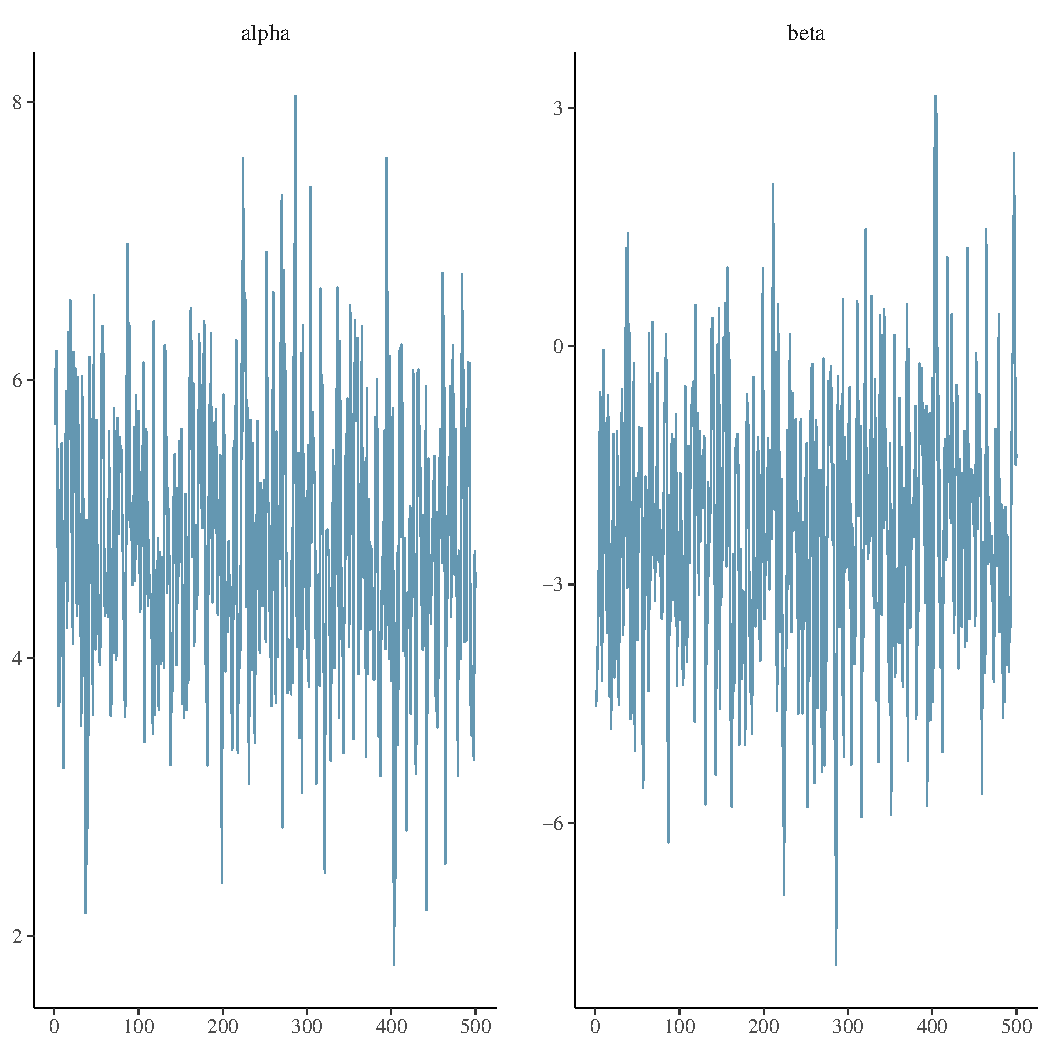
\includegraphics[width=\maxwidth]{figure/unnamed-chunk-6-1} 
\end{knitrout}

\newpage

\section*{A maybe...}


As an example, use data from (Gelman). Problem
consist of estimating the proportion of boys and girls.
Data: 251,527 boys and 241,945 girls born in Paris
from 1745 to 1770. Describe set up below

Privatize by adding noise, $\eta \sim N(0, 4000)$:
[Use DP framework?]
\begin{knitrout}
\definecolor{shadecolor}{rgb}{0.969, 0.969, 0.969}\color{fgcolor}\begin{kframe}
\begin{alltt}
\hlstd{n_g} \hlkwb{<-} \hlnum{241945}
\hlstd{n_b} \hlkwb{<-} \hlnum{251527}

\hlstd{eta} \hlkwb{<-} \hlkwd{rnorm}\hlstd{(}\hlnum{2}\hlstd{,}\hlnum{0}\hlstd{,}\hlnum{4000}\hlstd{)}

\hlstd{n_g} \hlopt{+} \hlstd{eta[}\hlnum{1}\hlstd{]}
\end{alltt}
\begin{verbatim}
## [1] 249361.9
\end{verbatim}
\begin{alltt}
\hlstd{n_b} \hlopt{+} \hlstd{eta[}\hlnum{2}\hlstd{]}
\end{alltt}
\begin{verbatim}
## [1] 247182.7
\end{verbatim}
\end{kframe}
\end{knitrout}

\subsection*{Sampling from likelihood under complete data}
binomial distribution
\begin{align*}
f(x \mid \theta) &= \binom{n}{n_g} \theta^{n_g}(1-\theta)^{n-n_g}
\end{align*}

\begin{knitrout}
\definecolor{shadecolor}{rgb}{0.969, 0.969, 0.969}\color{fgcolor}\begin{kframe}
\begin{alltt}
\hlstd{lik_smpl} \hlkwb{<-} \hlkwa{function}\hlstd{(}\hlkwc{theta}\hlstd{) \{}
  \hlstd{t1} \hlkwb{<-} \hlkwd{rbinom}\hlstd{(}\hlnum{1}\hlstd{,} \hlnum{493472}\hlstd{, theta)}
  \hlstd{t2} \hlkwb{<-} \hlnum{493472} \hlopt{-} \hlstd{t1}
  \hlkwd{c}\hlstd{(t1,t2)}
\hlstd{\}}
\end{alltt}
\end{kframe}
\end{knitrout}

\subsection*{Posterior given complete data}
Using Jeffrey's prior $Beta(1/2,1/2)$.
\begin{align*}
\dfrac{\Gamma(\alpha)\Gamma(\beta)}{\Gamma(\alpha + \beta)}x^{\alpha -1}(1-x)^{\beta-1}
\end{align*}
conjugate model:




\nocite{*}
\bibliographystyle{amsplain}
\bibliography{ref.bib}



\end{document}
